% !TeX program = xelatex
\documentclass{ctexart}
\usepackage[table]{xcolor}
\usepackage{template_by_mny}
\usepackage{float} 
\usepackage{listings}
\usepackage[figuresright]{rotating}
\lstset{basicstyle=\ttfamily, breaklines=true, frame=single}

\title{偏振实验报告}
\class{物理 32/物理 31}
\name{冯家琦/周方远}
\id{2023011338/2023011263}

\begin{document}

\maketitle

\section{引言}
本报告记录了使用偏振和3D电影技术套件进行的实验。这些实验旨在探索偏振原理、3D成像技术及其应用。
\section{实验原理}
\section{实验仪器}
\section{实验步骤}
\subsection{Part1:偏振实验}

\subsubsection{实验1:马吕斯定律}
在光路上依次摆放激光器、线偏振片1、线偏振片2、光强检测器。将两个偏振片的角度均调整为0。以4度为步长旋转第二个偏振片,记录光强检测器的电压值。

测量得到电压关于偏振片角度的数据如下图所示:
\begin{figure}[H]
    \centering
    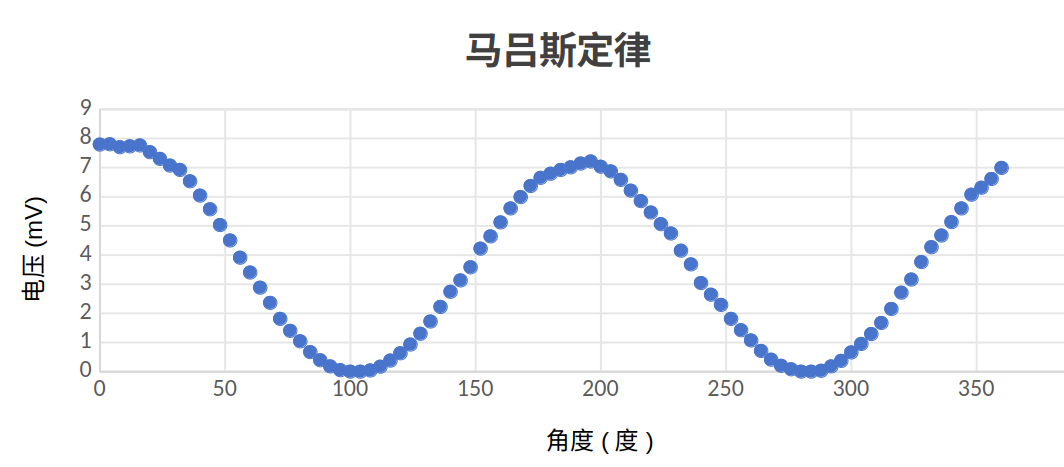
\includegraphics[width=0.8\textwidth]{实验一.png}
    \caption{电压-角度曲线}
\end{figure}

得到的数据曲线符合马吕斯定律。

\subsubsection{实验2:测量激光的偏振状态}
在光路上依次摆放激光器、线偏振片、光强检测器。从0度开始,以6度为步长旋转偏振片,记录光强检测器的电压。

测量得到电压关于偏振片角度的数据如下图所示:
\begin{figure}[H]
    \centering
    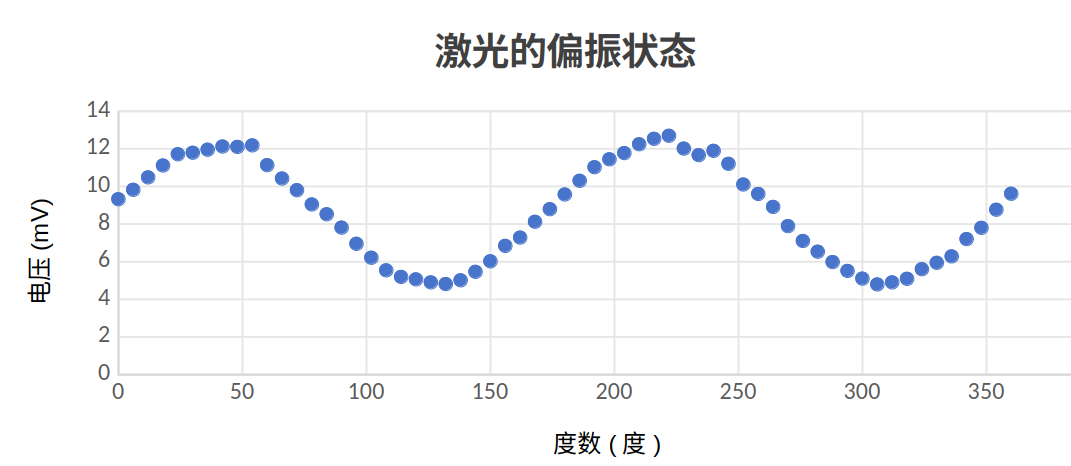
\includegraphics[width=0.8\textwidth]{实验二.png}
    \caption{电压-角度曲线}
\end{figure}
\begin{figure}[H]
    \centering
    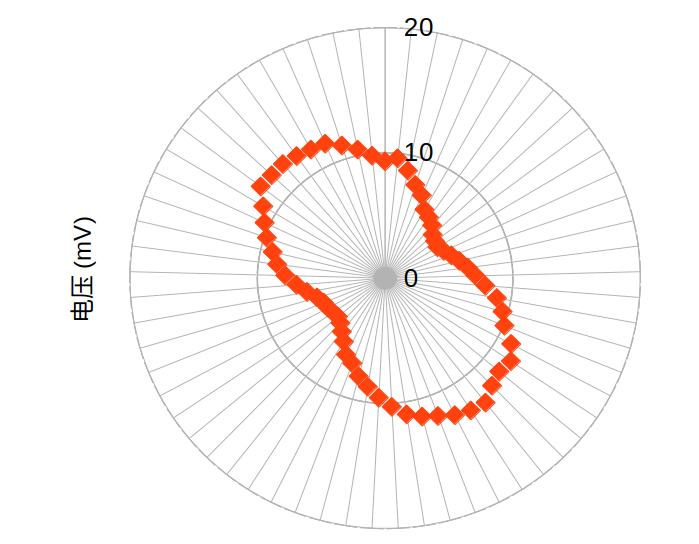
\includegraphics[width=0.6\textwidth]{实验二-2.png}
    \caption{上图在极坐标下的图像}
\end{figure}

从数据曲线中可以看出,激光器的偏振接近于线偏振。

\subsubsection{实验3:确定 $\lambda/4$ 板的取向}
在光路上依次摆放激光器、线偏振片1、$\lambda/4$片、线偏振片2、光强检测器。将两个线偏振片的偏振方向调为相互垂直。

缓慢旋转$\lambda/4$片,找到光强检测器能检测到的最大值和此时$\lambda/4$片的位置。此时$\lambda/4$片相较线偏振片正好旋过$45^\circ$。
\subsubsection{实验4:$\lambda/4$ 板对绿光的行为}
首先在激光器前放置一个偏振片,然后在其前面放置 $\lambda/4$ 板。$\lambda/4$ 板应相对于偏振片调整至 45°。现在证明绿激光在通过 $\lambda/4$ 板后变为圆偏振光。
\begin{figure}[H]
    \centering
    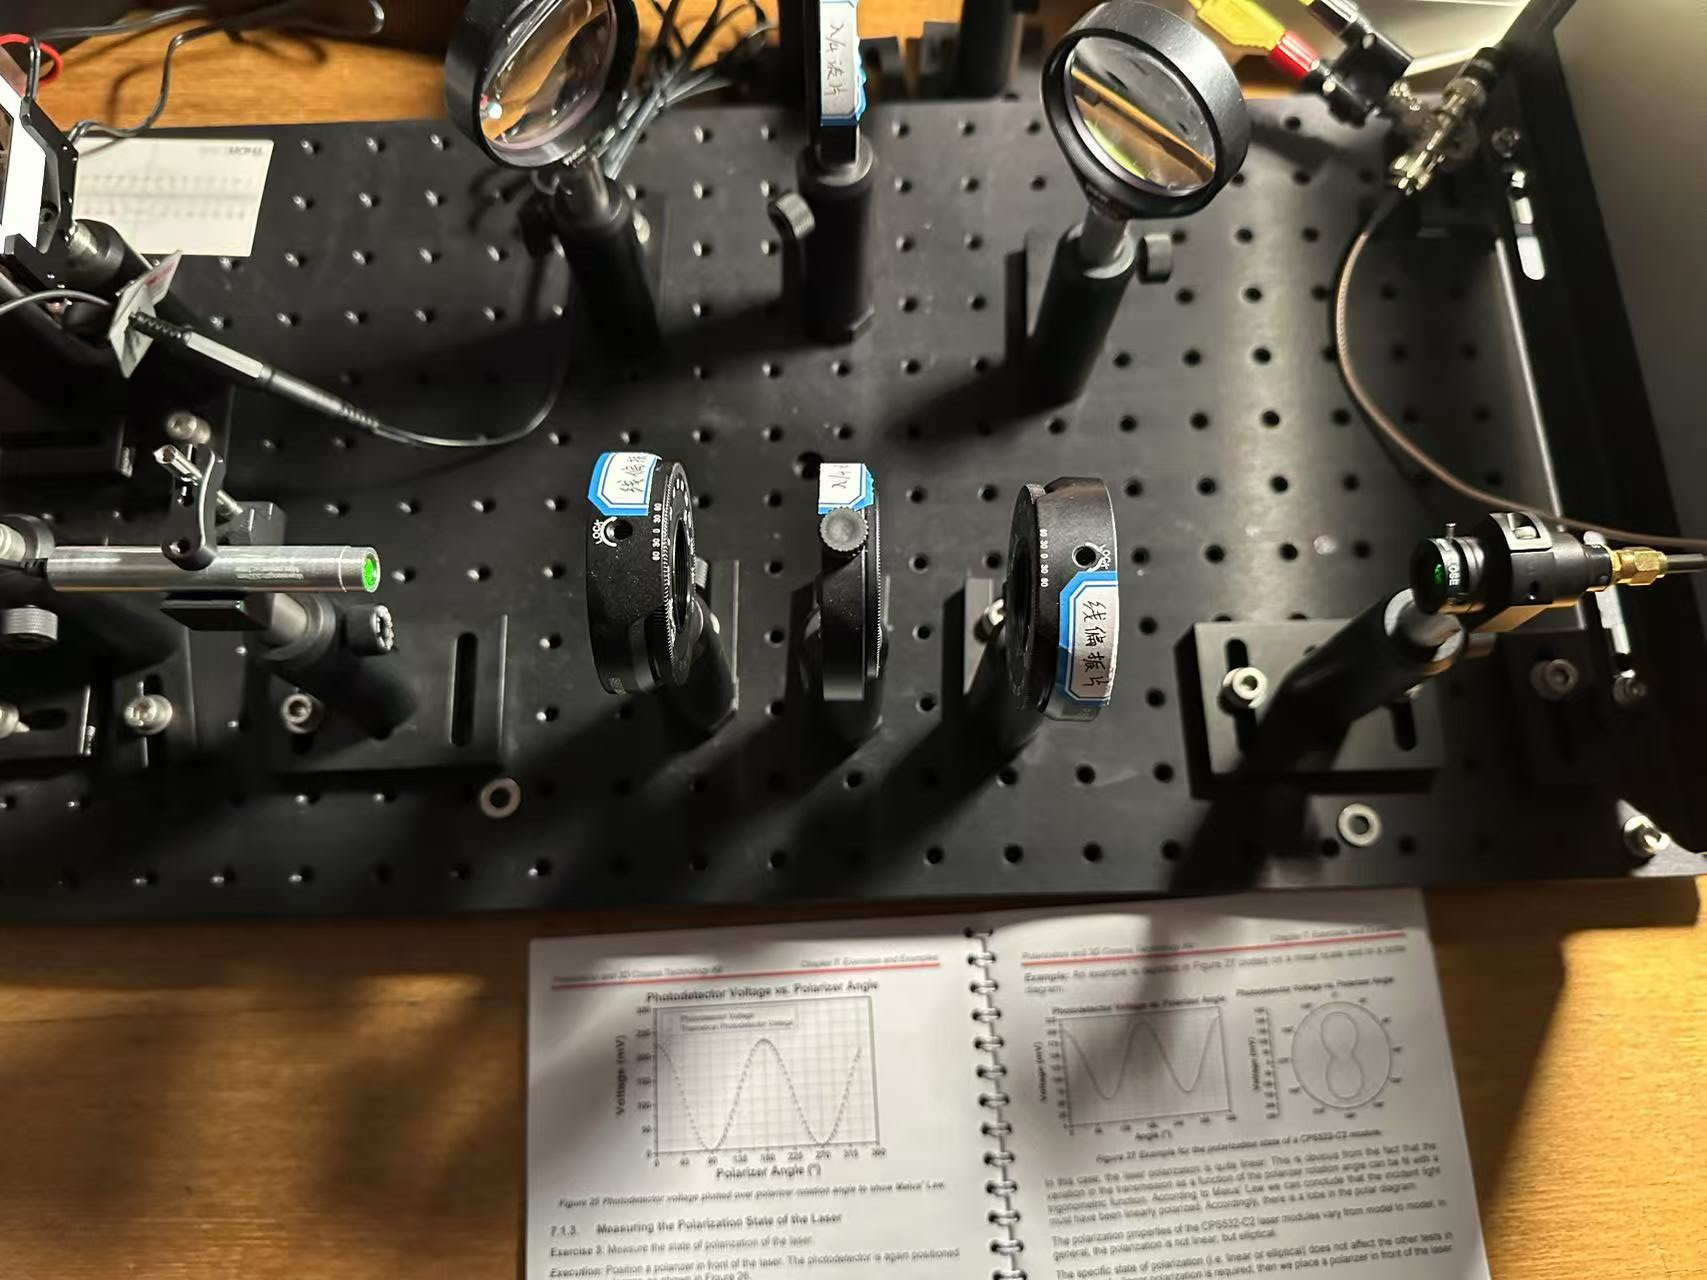
\includegraphics[width=0.4\textwidth]{偏振光路.png}
    \caption{实验4光路}
\end{figure}
调整第二个偏振器的角度,测量并记录对应的光强如下图所示
\begin{figure}[H]
    \centering
    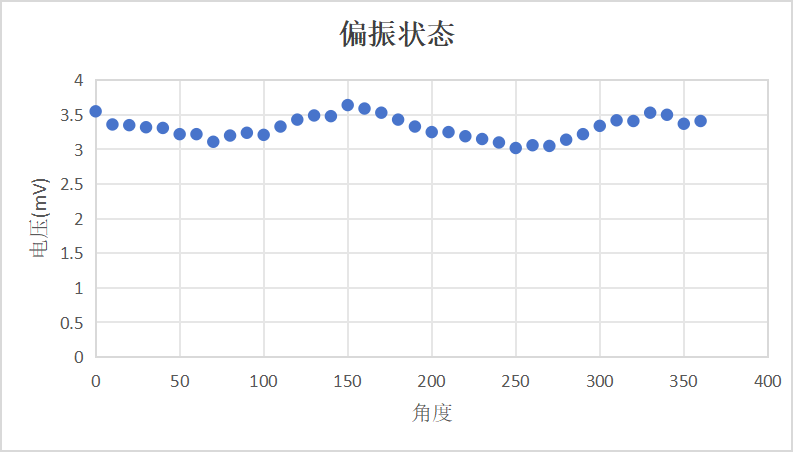
\includegraphics[width=0.5\textwidth]{实验5.png}
    \caption{实验5光强}
\end{figure}
可以看出,随着角度的变化,光强几乎不变

\subsubsection{实验5:糖量测定}
通过测量线性偏振光通过糖溶液时的偏振旋转角度,确定比例常数。

先在激光器前放两个相互垂直的线偏振片,然后在它们中间放一个玻璃容器,光路如图。
\begin{figure}[H]
    \centering
    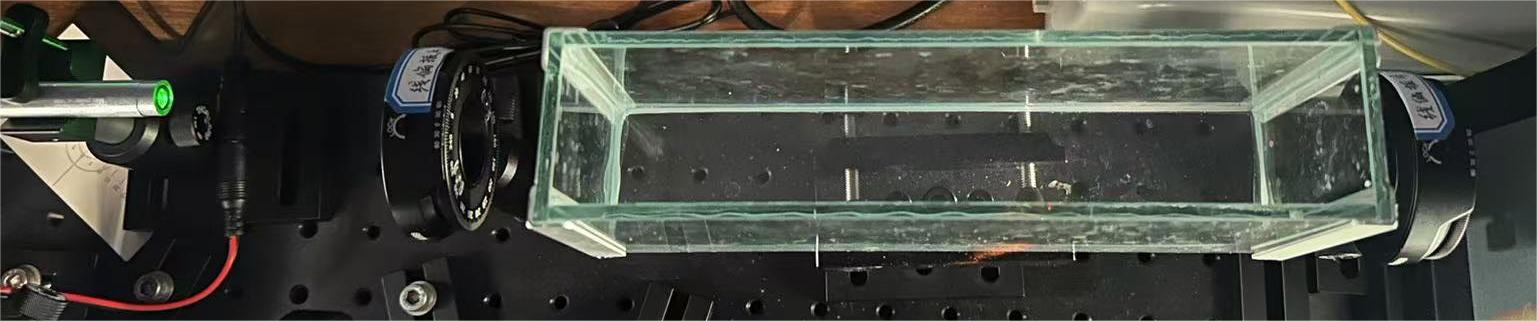
\includegraphics[width=0.7\textwidth]{糖光路(1).jpg}
    \caption{实验5光路}
\end{figure}
通过秤秤出22g糖并加入玻璃容器中,加入72mL水溶解。调整偏振片的角度使得光可以透过偏振片进入接受器,记录此时的角度。接下来如下图逐渐稀释糖溶液,记录每次稀释后的角度。
\begin{figure}[H]
    \centering
    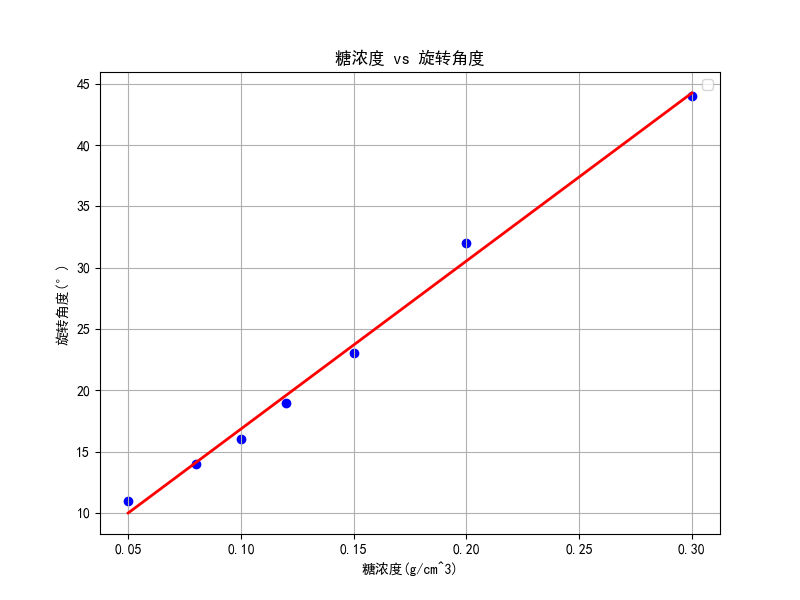
\includegraphics[width=0.5\textwidth]{糖浓度 vs 旋转角度.png}
\end{figure}
\end{document}